%%%%%%%%%%%%%%%%%%%%%%%%%%%%%%%%%%%%%%%%%
% "ModernCV" CV and Cover Letter
% LaTeX Template
% Version 1.11 (19/6/14)
%
% This template has been downloaded from:
% http://www.LaTeXTemplates.com
%
% Original author:
% Xavier Danaux (xdanaux@gmail.com)
%
% License:
% CC BY-NC-SA 3.0 (http://creativecommons.org/licenses/by-nc-sa/3.0/)
%
% Important note:
% This template requires the moderncv.cls and .sty files to be in the same 
% directory as this .tex file. These files provide the resume style and themes 
% used for structuring the document.
%
%%%%%%%%%%%%%%%%%%%%%%%%%%%%%%%%%%%%%%%%%

%----------------------------------------------------------------------------------------
%	PACKAGES AND OTHER DOCUMENT CONFIGURATIONS
%----------------------------------------------------------------------------------------

\documentclass[10pt,a4paper,sans]{moderncv} % Font sizes: 10, 11, or 12; paper sizes: a4paper, letterpaper, a5paper, legalpaper, executivepaper or landscape; font families: sans or roman

\usepackage[utf8]{inputenc}

\usepackage[export]{adjustbox}

\usepackage{multicol}

\usepackage{pbsi}

\usepackage{datetime}

\moderncvstyle{casual} % CV theme - options include: 'casual' (default), 'classic', 'oldstyle' and 'banking'
\newcommand{\colorName}{blue}
\moderncvcolor{\colorName} % CV color - options include: 'blue' (default), 'orange', 'green', 'red', 'purple', 'grey' and 'black'

\usepackage{color}

\usepackage{lipsum} % Used for inserting dummy 'Lorem ipsum' text into the template

\usepackage[scale=0.90]{geometry} % Reduce document margins
\setlength{\hintscolumnwidth}{4cm} % Uncomment to change the width of the dates column
%\setlength{\makecvtitlenamewidth}{10cm} % For the 'classic' style, uncomment to adjust the width of the space allocated to your name

%----------------------------------------------------------------------------------------
%	NAME AND CONTACT INFORMATION SECTION
%----------------------------------------------------------------------------------------

\firstname{Furkan} % Your first name
\familyname{KARAKAŞ} % Your last name

\title{Curriculum Vitae}

%----------------------------------------------------------------------------------------

\begin{document}

\textit{\Huge{\textcolor{gray}{Curriculum Vitae}}}

\hrulefill
%----------------------------------------------------------------------------------------
%	PERSONAL SECTION
%----------------------------------------------------------------------------------------

\begin{multicols}{2}
  \section{Personal Information}
  \cvitem{Name}{Furkan KARAKAŞ}
  \cvitem{Date of Birth}{\emph{August 24th, 1995}}
  \cvitem{Birthplace}{Istanbul}
  \cvitem{Address}{Breite 2, 5210 Windisch, Switzerland}
  \cvitem{Mobile}{+41 77 915 99 35}
  \cvitem{E-Mail}{\href{mailto:furkan.karakas@epfl.ch}{furkan.karakas@epfl.ch}}
  \cvitem{Personal Website}{\url{https://furkankarakas.github.io/}}
  \cvitem{GitHub}{\url{https://github.com/FurkanKarakas}}
  \cvitem{LinkedIn}{\url{https://www.linkedin.com/in/furkan-karakas/}}
  \cvitem{Civil Status}{Single}
  \cvitem{Nationality}{Turkey}
  \columnbreak
  \hspace{-0.05\textwidth}
  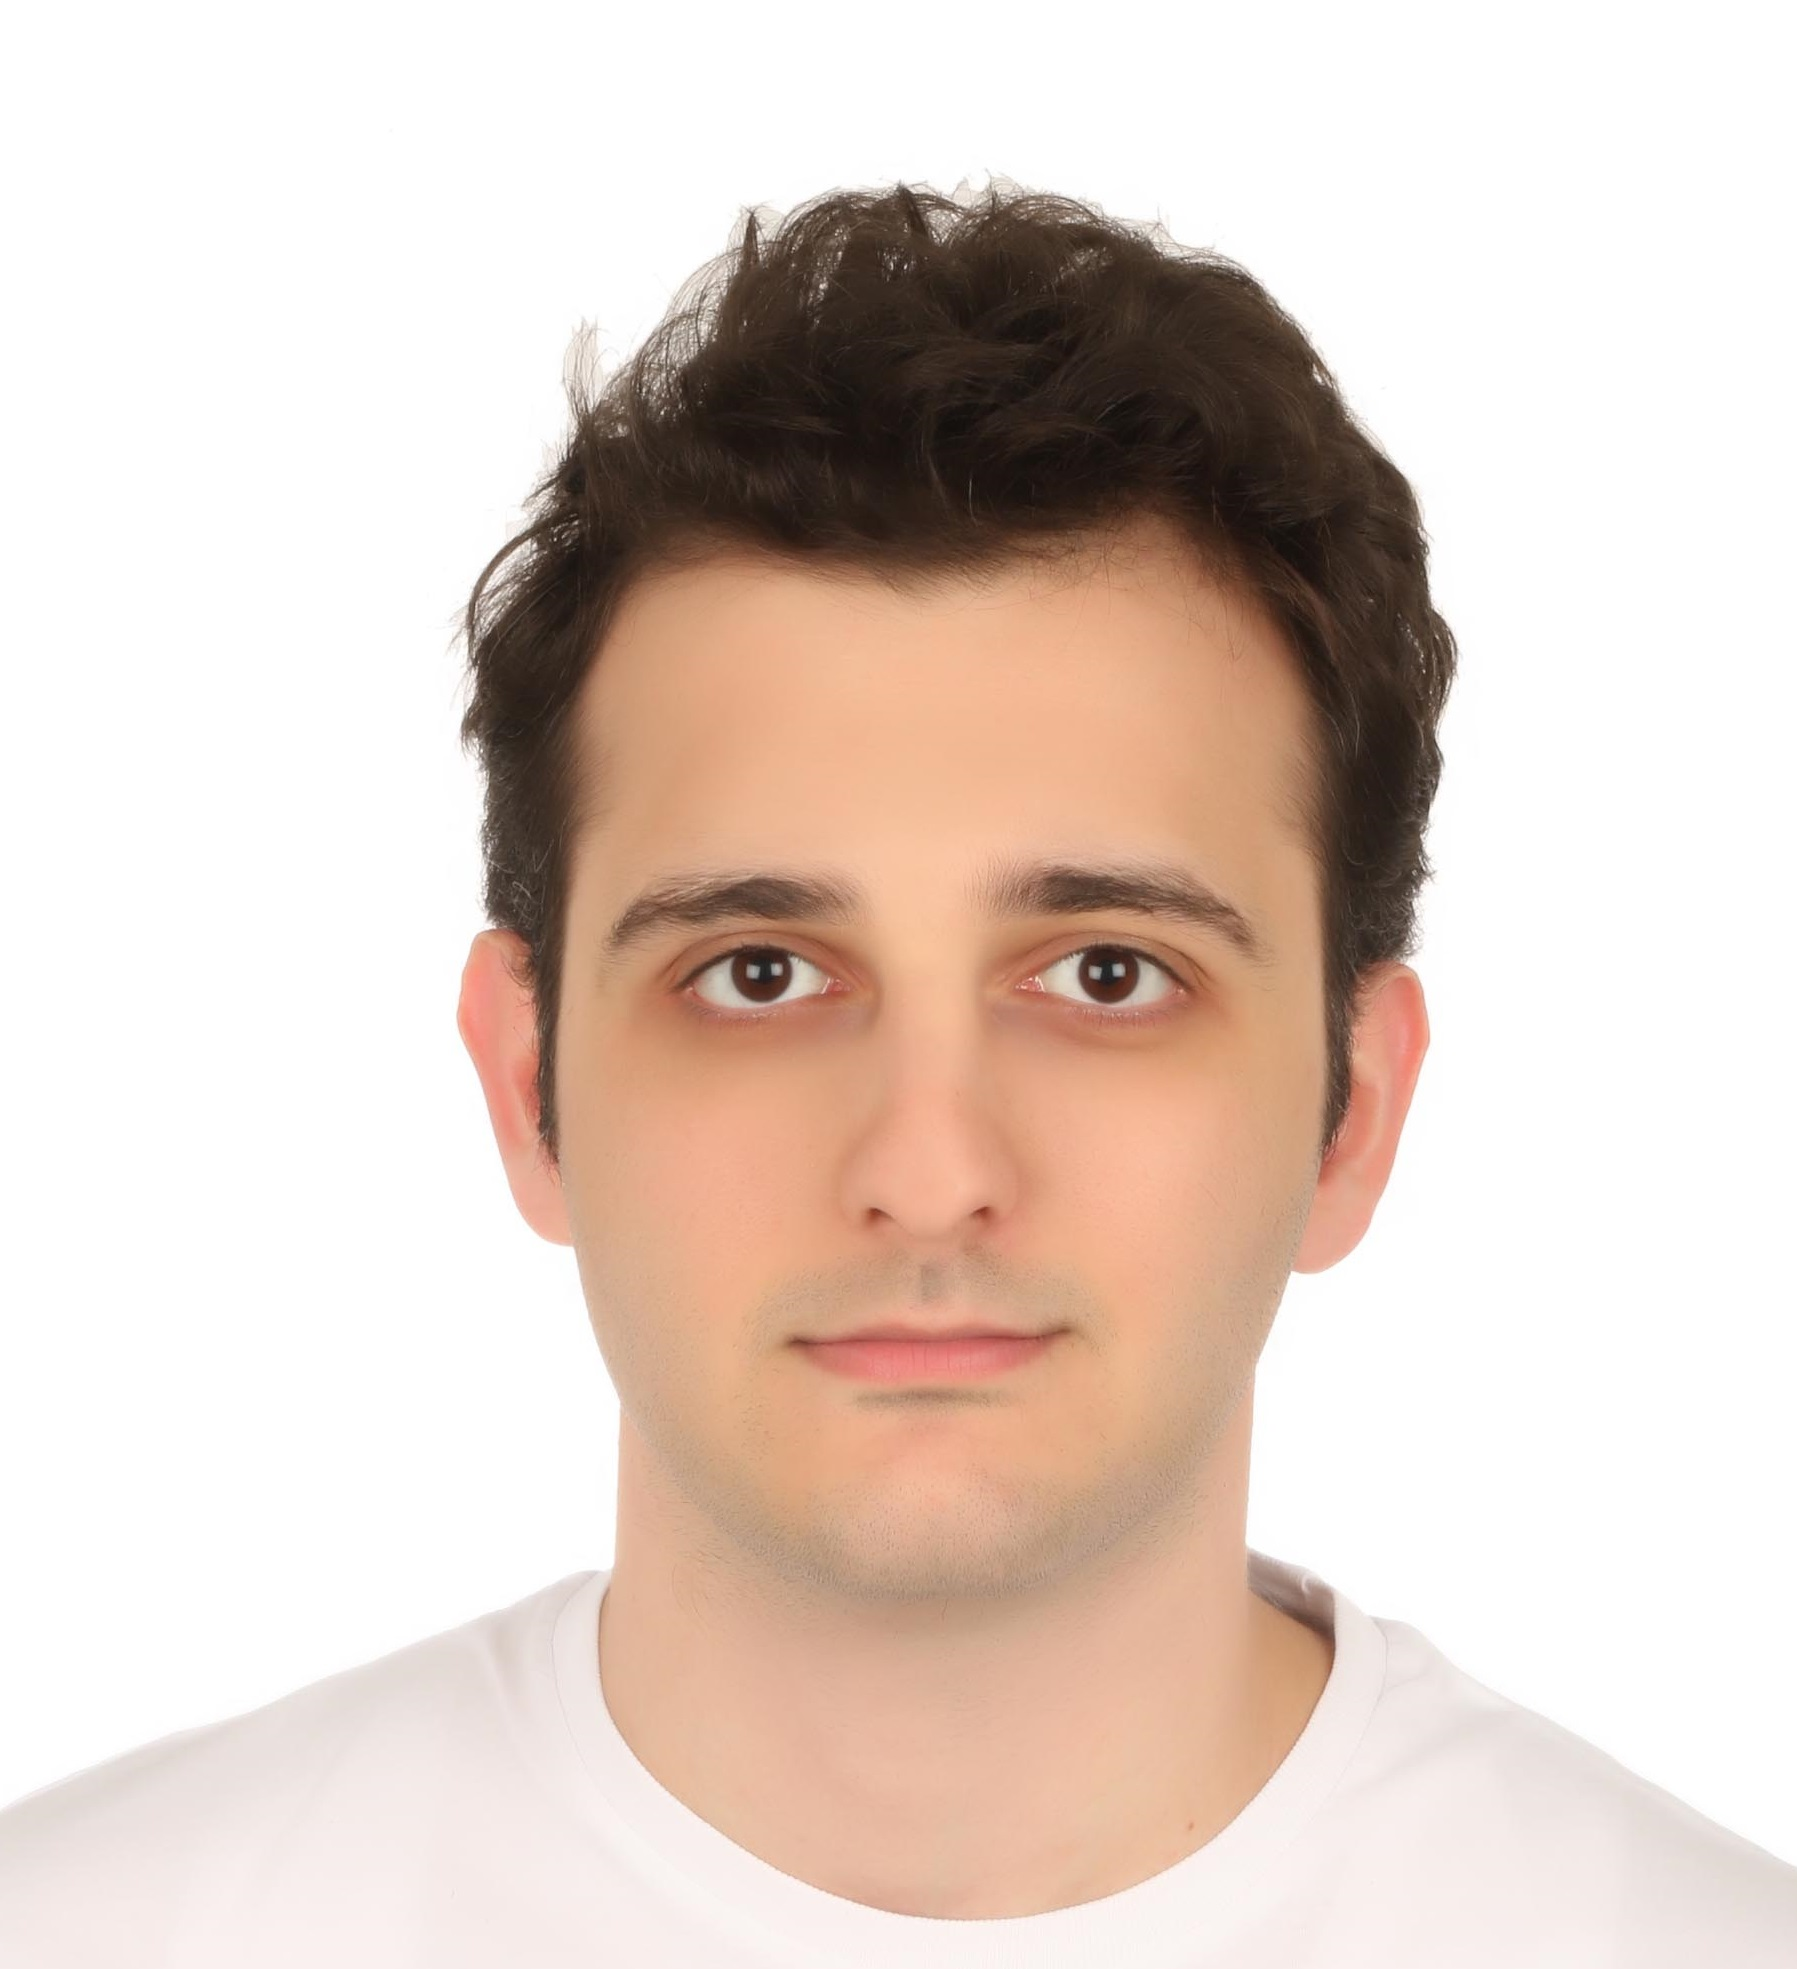
\includegraphics[width=31mm, right]{pictures/furkan_vize.jpg}
\end{multicols}

%----------------------------------------------------------------------------------------
%	OBJECTIVE SECTION
%----------------------------------------------------------------------------------------

\section{Objective}

\cvitem{}{Looking for positions in}
\cvlistitem{distributed computing,}
\cvlistitem{networking,}
\cvlistitem{cryptography and security,}
\cvlistitem{blockchain technologies, or}
\cvlistitem{Internet of Things.}

%----------------------------------------------------------------------------------------
%	EDUCATION SECTION
%----------------------------------------------------------------------------------------

\section{Education}

\cvitem{Sep 2019 -- Present}{\textbf{Swiss Federal Institute of Technology} \textit{Lausanne, Switzerland} \newline Msc. in communication systems, specialization in cyber security \textit{Current GPA: 5.29/6.00}}
\cvlistitem{\textbf{Teaching assistant} of the fourth semester bachelor course \textit{Signals and Systems} in \textit{Spring 2020}}

\cvitem{Apr 2018 -- Sep 2018}{\textbf{Technical University of Munich} \textit{Munich, Germany} \newline Erasmus+ exchange studies}

\cvitem{Feb 2015 -- Jul 2019}{\textbf{Boğaziçi University} \textit{Istanbul, Turkey} \newline Bsc. in electrical \& electronics engineering, double major with the department of mathematics, graduation with high honor certificate \textit{GPA: 3.59/4.00}}

\cvitem{Sep 2009 -- Jun 2014}{\textbf{Istanbul High School} \textit{Istanbul, Turkey} \newline German high school}


%----------------------------------------------------------------------------------------
%	WORK EXPERIENCE SECTION
%----------------------------------------------------------------------------------------

\renewcommand{\listitemsymbol}{\textcolor{black}{-~}} % Changes the symbol used for lists

\section{Work Experience}

\cvitem{Jul 2020 -- Present}{\textbf{ABB Corporate Research Center} \textit{Baden, Switzerland} -- Student Internship} 
\cvlistitem{Working on a project to store the values generated by IoT sensors in a blockchain platform in a secure fashion}
\cvlistitem{\textit{Hyperledger Fabric} as the underlying private and permissioned blockchain system}
\cvlistitem{Building a front-end \textit{React.js} application to interact with the blockchain system}

\cvitem{Aug 2019 -- Jan 2020}{\textbf{Albert Solino Consultancy} \textit{California, USA} \url{https://albertsolinocorp.com/} -- Junior Web Application Developer}
\cvlistitem{Working remotely on a web application development}
\cvlistitem{Consultancy services in a digital platform}
\cvlistitem{Performance calculation logic}
\cvlistitem{Working in the back-end part in Ruby on Rails platform}
\cvlistitem{Using standard Model-View-Controller (MVC) architectural pattern}

\cvitem{Apr 2019 -- Jul 2019}{\textbf{Arçelik Global} \textit{Istanbul, Turkey} \url{http://www.arcelikglobal.com/} -- Project Assistant}
\cvlistitem{Assisted my team in a project concerning smart-home devices}
\cvlistitem{Preparation of checklists for the components}
\cvlistitem{Sensor virtualization in C so that one could send virtual inputs to the components rather than reading from physical sensors}

\cvitem{Jun 2018 -- Sep 2018}{\textbf{CAX-SERVICE GmbH Software-Engineering \& Messtechnik} \textit{Munich, Germany} \url{http://www.cax-service.org/} -- Part-time Working Student}
\cvlistitem{Assisted as a freelancer in developing various software in .NET framework C\#}
\cvlistitem{Windows form applications}

\cvitem{Jun 2018 -- Sep 2018}{\textbf{Wörner Medizinprodukte und Logistik GmbH} \textit{Munich, Germany} -- Part-time Working Student}
\cvlistitem{Accounting, documentation, preparation of Excel sheets, data analysis in Excel}

\cvitem{Feb 2018 -- Mar 2018}{\textbf{Accelera Software and Consultancy} \textit{Istanbul, Turkey} \url{http://www.accelera.com.tr/contact/} -- Internship}
\cvlistitem{Internship about data mining, machine learning, SQL, and R}
\cvlistitem{Application of supervised and unsupervised algorithms to business solutions: random forests, linear regressions, logistic trees, etc.}

%----------------------------------------------------------------------------------------
%	EXTRACURRICULAR SECTION
%----------------------------------------------------------------------------------------

%----------------------------------------------------------------------------------------
%	SKILLS SECTION
%----------------------------------------------------------------------------------------
%\vspace{14mm}
\section{Skills \& Background Knowledge}

\subsection{Technical skills}

\cvitem{}{C, Python \textit{Advanced}}
\cvitem{}{C\#, C++, \LaTeX, MATLAB, Golang \textit{Intermediate}}
\cvitem{}{Java, HTML, CSS, JavaScript, Node.js, React, Web development technologies \textit{Beginner}}
\cvitem{}{Version control systems (Git)}
\cvitem{}{Basic knowledge of the Linux operating system}
\cvitem{}{VS Code (My favorite code editor)}



%----------------------------------------------------------------------------------------
%	COMMUNICATION SKILLS SECTION
%----------------------------------------------------------------------------------------

\subsection{Personal skills}

\cvitem{}{High level in communication skills}
\cvitem{}{Sociable and proactive}

%----------------------------------------------------------------------------------------
%	LANGUAGES SECTION
%----------------------------------------------------------------------------------------

\section{Languages}

\renewcommand{\listitemsymbol}{\textcolor{\colorName}{o~}}

\cvitem{}{English, \textit{C2}}
\cvlistitem{TOEFL iBT Internet-based examination score \textit{102} out of \textit{120}}
\cvitem{}{German, \textit{C1}}
\cvlistitem{Abitur Diploma \textit{1.9/4.0} (1.0 is the best score in the German system)}
\cvitem{}{French, \textit{A1}}
\cvitem{}{Turkish, \textit{Mother Tongue}}


%----------------------------------------------------------------------------------------
%	INTERESTS SECTION
%----------------------------------------------------------------------------------------

\section{Interests}

\renewcommand{\listitemsymbol}{-~} % Changes the symbol used for lists

\cvlistitem{Computer games, mainly multi-player ones such as Massively multiplayer online role-playing games (MMORPGs) and Multiplayer online battle arenas (MOBAs)}
\cvlistitem{Gym \& Fitness}
\cvlistitem{Constantly learning new things in the IT world}

\section{References}
\cvitem{}{Available upon request}

\vspace{8mm}

\begin{flushright}
{\fontfamily{qcr}\selectfont
Furkan Karakaş, Windisch, \today
}
\end{flushright}
\hspace{.70\textwidth}

\includegraphics[width=20mm]{pictures/imza.jpg}

\end{document}